\documentclass[a4paper]{article}

%% Language and font encodings
\usepackage[english]{babel}
\usepackage[utf8x]{inputenc}
\usepackage[T1]{fontenc}

%% Sets page size and margins
\usepackage[a4paper,top=3cm,bottom=2cm,left=3cm,right=3cm,marginparwidth=1.75cm]{geometry}

%% Useful packages
\usepackage{amsmath}
\usepackage{graphicx}
\usepackage[colorinlistoftodos]{todonotes}
\usepackage[colorlinks=true, allcolors=blue]{hyperref}

\title{ACM Winter Workshop: Summary}
\author{-Dimpy Chhabra}

\begin{document}
\maketitle

\section{Introduction}
The ACM-IGDTU student chapter conducted a five day workshop on data science and machine learning. 
The workshop included of working with the Twitter API, Facebook API, for data collection, preparation and data analysis in R, and machine learning concepts and applications using Scikit learn in python.
Guest lecturers from Precog were invited to take various sessions too.
The workshop culminated in a project discussion seminar and certificate distribution ceremony.

\section{What did we learn?}
Over the course of five days we went through the following laid out curriculum:

\begin{itemize}
\item Registration and Preparing Computing Environment
\item Preliminaries: Python and R
\item Data Collection from Social Media Platforms
\item Issues and Challenges in Data Collection
\item Data Analysis: Univariate and Bivariate
\item Data Visualization
\item Graph Data Analysis
\item Application of Data Analysis
\item Data Distributions, Parameter Estimation
\item Hypothesis Testing
\item Research Skills: Reading and Documentation
\item Applications in Real World Problems
\item Supervised Learning
\item Regression
\item Unsupervised Learning
\item Applications of Machine Learning
\item Key Research Areas
\item Hearing from Participants
\item Certificate Distribution and Valedictory Ceremony
\end{itemize}

\subsection{Day 1 Takeaways }

Data Collection:
	
\begin{itemize}
\item Datasets\newline
 		==>Ques Uno. Data Entities and attributes.\newline
 		==>Publically Available\newline
\item 	APIS\newline
		==>Website's provide with API Access.\newline
 		==>Ex. Graph API(Facebook)\newline
\item 	Web Scraping\newline
 		==>Scraping the internet\newline
\item 	Selenium\newline
		==>Automating handled here
\end{itemize}
Above is the exhaustive list of getting data!
Thus, one must be able to work on getting data out of APIs or the internet in general.

\begin{figure}
\centering
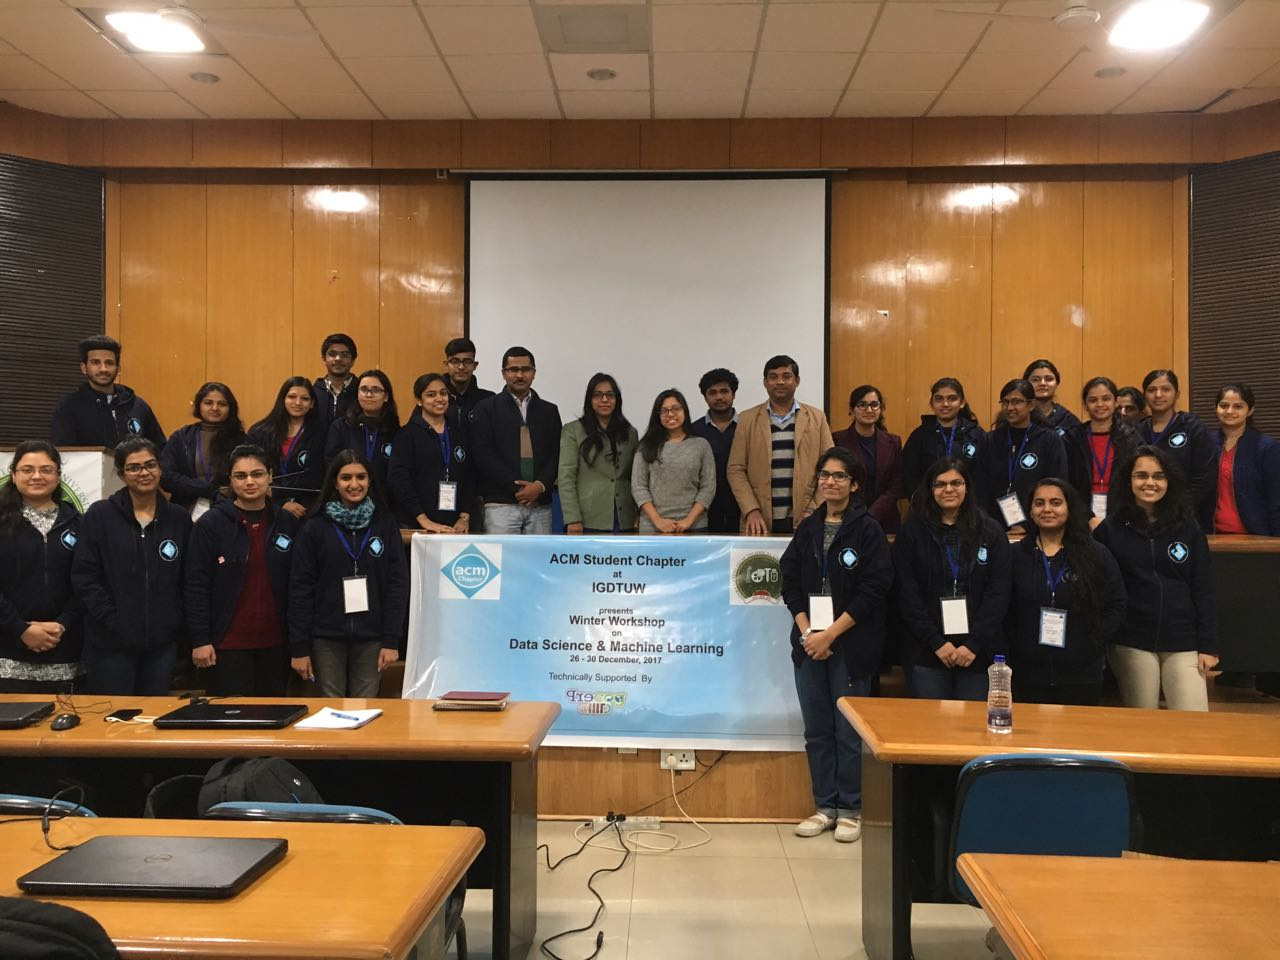
\includegraphics[width=0.9\textwidth]{ACM_Winter_Workshop_group_photo.jpg}
\caption{\label{fig:acm}Day 5 ceremony.}
\end{figure}
\subsection{Day 2 Takeaways }

On our second day we discussed various concepts: \newline
	
\begin{itemize}
\item Data Representation\newline
 		We learnt about the matrix representation of data. ie. Data can be presented in a data Matrix in two dimension that is n and d. where the coloumns are the attributes and the rows are the tuples! Further discussed the two broad classifications of attributes: Numerical and Categorical. We also discussed the two viewpoints: Probabilistic and Algebraic 'nd Geometric.\newline
        Thusly leading into various distributions like Bernoulli, binomial, normal and Poisson. 
\item 	Analysis: Univariate and Bivariate\newline
		Waltz through the various univariate analysis like mean, mode and median; followed by implementation on IRIS dataset in R language.\newline
        In the latter we discussed correlation and thusly, the development of graphs out of datasets on the basis of similarity degrees.
\item 	Graph Data Analysis\newline
 		Studied degree distributions, walks, paths, connectedness, graph representations etc, to eventually dwell into developing similarity graphs. ex. Gaussian Similarity graph for Iris dataset.\newline
        Ideas like \newline 
        -> Clustering Coefficient\newline
        -> Centrality Analysis \newline
		-> Eccentricity Analysis \newline
		-> Closeness Centrality\newline
       were discussed with real time possible applications of each, simply based on the twitter network.
        
\item 	Other Topics discussed included of:\newline
		==> Baseline // GroundTruth \newline
        ==> Small World Property and Ultra Small World Property\newline
        ==> Power Law Relationship
\end{itemize}

\subsection{Day 3 Takeaways }

Day 3 included of detailed discussions and uses of various distributions. Namely, Bernoulli, binomial, Poisson and Normal. \newline
This discussion was followed by the Hypothesis testing, and a simple hands-on session on git and github.
	
\subsection{Day 4 Takeaways }

On our fourth day we went head-first into machine learning. Theoretical sessions were followed by hand-on sessions, where we worked in python using Scikit learn. \newline
The codes and representation of the work done can be found  \href{https://github.com/dimpy-chhabra/ACM_Winter_Workshop/tree/master/Day_4/Scikit-Learn}{here}.

\subsection{Day 5 Takeaways }

Certificate Ceremony and a session on 'how to read and write research papers', thus studying \cite{greenwade93} \newline
The pictures of the same can be found  \href{https://drive.google.com/drive/folders/17kIdg3UKXfFie57A472nyZtZ7WvmDR4E}{here}.
	

\section{Conclusion}
On and All, the workshop was a great learning experience!
The various assignment problems and my solutions can be found on my github portal \href{https://github.com/dimpy-chhabra/ACM_Winter_Workshop}{here}.
\newline

%
%You can upload a \verb|.bib| file containing your BibTeX entries, created with JabRef; or import your \href{https://www.overleaf.com/blog/184}{Mendeley}, CiteULike or Zotero library as a \verb|.bib| file. You can then cite entries from it, like this: \cite{greenwade93}. Just remember to specify a bibliography style, as well as the filename of the \verb|.bib|.

Reach me @
\url{http://www.dimpychhabra.co} :)

\bibliographystyle{alpha}
\bibliography{sample}

\end{document}